\question (华中科技大学,2007年)具有6个顶点的无向图,至少有(
)条边时能确保是一个连通图
\par\twoch{8}{9}{10}{\textcolor{red}{11}}
\begin{solution}首先5个顶点最多占10个边(4+3+2+1),再加一条边就能把第六个顶点连通到这个图里。故最少需要10+1=11条边,便可保证6个顶点的连通。
\end{solution}
\question (华南理工大学,2005年)以下有关图的叙述中,正确的是( )
\par\fourch{强连通有向图的任何顶点到其他所有顶点都有弧}{任意图顶点的入度等于出度}{\textcolor{red}{有向完全图一定是强连通有向图}}{有向图的边集的子集和顶点集的子集可构成原有向图的子图}
\begin{solution}强连通有向图是指对于每一对顶点vi和vj,从vi到vj和从vj到vi都有路径,而不是都有弧,因此A错误。
绝大部分有向图的入度都不等于出度,因此B错误。
C是正确的,有向完全图,任一两个顶点都有两条边相连,可推出对于每一对顶点vi和vj,从vi到vj和从vj到vi都有路径,因此有向完全图一定是强连通有向图。
假设边集选了某个边a,顶点集没选a边的两个顶点,则构不成图,更别说是其子图了,因此D错误。
\end{solution}
\question (上海交通大学,2005年)在无向图中定义顶点Vi与Vj之间的路径为从Vi到达Vj的一个(
)
\par\twoch{\textcolor{red}{顶点序列}}{边序列}{权值总和}{边的条数}
\begin{solution}路径是一个顶点序列。
\end{solution}
\question (北京邮电大学,2007年)一个具有n个顶点的连通无向图,最少有( )条边
\par\twoch{\textcolor{red}{n-1}}{n}{n(n-1)/2}{n(n-1)}
\begin{solution}考虑两个点的情况,只需要一条边就可以连通。以后每加入一个点,只需要加入一条边就可将其连通,因此我们可以得出n-1条边就能够把n个顶点连通了,至于有没有更少的情况我们不用证明。因为B、C和D给出的表达式都比n-1大,因此排除B、C和D,本题选A。
\end{solution}
\question (南京邮电大学,2006年)下面的( )算法可用于求无向图的所有连通分量
\par\twoch{\textcolor{red}{广度优先遍历}}{拓扑排序}{求最短路径}{求关键路径}
\begin{solution}从图中的一个顶点进行广度优先搜索可以将与这个顶点连通的顶点全部都遍历到,也就找到了该顶点所在的连通分量,因此广度优先遍历可以求出无向图的所有连通分量。
拓扑排序是针对有向图而言的,无向图没法进行拓扑排序,排除B。
最短路径和关键路径都只能遍历到部分顶点,排除C、D。
\end{solution}
\question 下列关于无向连通图特性的叙述中 ,正确的是( )。
\ding{192}.所有顶点的度之和为偶数 \ding{193}.边数大于顶点个数减1
\ding{194}.至少有一个顶点的度为1
\par\twoch{\textcolor{red}{只有\ding{192}}}{只有\ding{193}}{\ding{192}和\ding{193}}{\ding{192}和\ding{194}}
\begin{solution}在无向图中,一条边在度之和中计为2,所以度之和为边数的2倍,\ding{192}正确。
无向连通图边数最少时为树图的情况,此时边数为顶点个数减1,\ding{193}错误。
\ding{194}错误,例如一个连接所有顶点的环,边数等于顶点个数,每个顶点的度都是2。
【总结】
本题属于概念理解性题目,难度并不大,只要理解无向图和连通图的概念即可容易求解。
① 直观来说,若一个图中每条边都是无方向的,则称为无向图。 ②
在一个无向图G中,若从顶点vi到顶点vj有路径相连(当然从vj到vi也一定有路径),则称vi和vj是连通的。如果G是有向图,那么连接vi和vj的路径中所有的边都必须同向。如果图中任意两点都是连通的,那么图被称作连通图。
\end{solution}
\question 下列关于图的叙述,正确的是( )。 \ding{192}.回路是简单路径
\ding{193}.存储稀疏图,用邻接矩阵比邻接表更省空间
\ding{194}.若有向图中存在拓扑序列,则该图不存在回路
\par\twoch{仅\ding{193}}{仅\ding{192}、\ding{193}}{\textcolor{red}{仅\ding{194}}}{仅\ding{192}、\ding{194}}
\begin{solution}若路径中除了开始点和结束点可以相同以外,其余顶点均不相同,则称这条路径为简单路径。若一条路径中第一个顶点和最后一个顶点相同,则这条路径是一条回路(回路中可能存在既不是起点也不是终点的相同点),故\ding{192}错误。后话,要是两者是充要条件,也就不必要两个名词了。
邻接矩阵无论图是稀疏还是稠密,都取的是最大的存储空间,因此用邻接表比邻接矩阵更省空间,故\ding{193}错误。
用拓扑排序的方法可以判断图中是否存在回路,如果对一个图可以完成拓扑排序,则此图不存在回路,故\ding{194}正确。
【总结】
本题考查了图的多个知识点,但本题目出的不是很好,属于3个比较简单的判断题的生硬拼凑,不能算是好的``综合''题。但做题的同学需要掌握多个基础知识点才可正确解答。
\end{solution}
\question 若无向图G=(V,E)中含有7个顶点,要保证图G在任何情况下都是连通的,则需要的边数最少是(
)
\par\twoch{6}{15}{\textcolor{red}{16}}{21}
\begin{solution}要保证无向图G在任何情况下都是连通的,即任意变动图G中的边,G始终保持连通,首先需要G的任意六个结点构成完全连通子图G1,需15条边(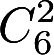
\includegraphics[width=0.19792in,height=0.19792in]{texmath/4a64ea5Cdpi7B3507DC_65E2}),然后再添一条边将第7个结点与G1连接起来,共需16条边。
【总结】
本题重在对题意的理解上面,保证图G在任何情况下都是连通的,需要多少边数。而不是连通图最少需要多少边数。理解了题意,就知道其实考查的是完全连通图。加上一条边即可。
对于具有n个顶点的无向图,当其中n-1个顶点构成一个完全图时,再加上任一条边必然构成一个连通图,所以最少边数=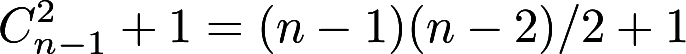
\includegraphics[width=2.44792in,height=0.19792in]{texmath/1a7ad05Cdpi7B3507DC_7Bn-17D5E22B13D28n-12928n-2292F22B1}。
\end{solution}
\question 设图的邻接矩阵A如下图所示。各顶点的度依次是( ~)。~

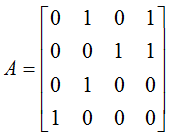
\includegraphics[width=1.77083in,height=1.43750in]{computerassets/596518D94738A905011156D7D79F7DEE.png}
\par\fourch{1,2,1,2}{2,2,1,1}{\textcolor{red}{3,4,2,3}}{4,4,2,2}
\begin{solution}各顶点的度包括了入度和出度,因此是矩阵中此结点对应的横行和纵列非零元素之和,所以可得各顶点的度分别为3,4,2,3。
\end{solution}
\question (中南大学,2004年)一个有28条边的非强连通无向图至少有( )个顶点
\par\twoch{7}{8}{\textcolor{red}{9}}{10}
\begin{solution}因为8个顶点的强连通无向图共有8*(8-1)/2=28个顶点,所以非强连通无向图则至少有9个节点
\end{solution}
\question (北京邮电大学,2004年)对于有n个顶点e条边的连通图,其生成子图边的最小数目是(
)
\par\twoch{0}{n}{\textcolor{red}{n-1}}{e}
\begin{solution}生成子图最小的边的数目是这个图的生成树的边的数目,即为n-1
\end{solution}
